% ##################################################################################################################
\chapter{London}
\label{ch:london}
\hfill \textbf{Authors:} Joan Serras, Melanie Bosredon, Vassilis Zachariadis, Camilo Vargas-Ruiz, Thibaut Dubernet, Mike Batty

% ##################################################################################################################
The building of a travel demand model for London started to take shape under the EUNOIA Project\footnote{see \url{http://eunoia-project.eu}}. 
The core decisions around the model design were taken after two meetings with \gls{tfl}, which was part of the Advisory Board in the project. 
In that respect, the main suggestion by \gls{tfl} was the adoption of an activity-based approach.

The main traits from the current implementation of the London model are listed next:
%
\begin{itemize}\styleItemize
\item Our baseline year is 2010.
\item	The geographic extent of the case study area is contained within the M25 and includes around 9,4\,million inhabitants (Census~2011)
\item	The types of activity included in the model are: home, work, shop, education, leisure and other.
\item	Four travel modes have been included: walk, cycle, car and public transport. The public transport mode includes buses, underground, rail, the Docklands Light Railway and the London Overground.
\item	The zones of analysis for the London model are the English Census~2011 Wards which we will refer to as wards from now on. Our case study is composed of 850\,wards.
\end{itemize}
%
% ##################################################################################################################
\section{Supply}
The assembly of the supply for our model includes the definition of the following three components:
%
\begin{itemize}\styleItemize
\item	Road network
\item	Public transport services
\item	Land-use configuration
\end{itemize}
%
The data used to build the road network is the Integrated Transport Network from the Ordnance Survey. 
The source network, which is defined at the navigation level, has been processed to remove some of the detail included. 
Decisions on the capacity of each road link has been based on the guidelines proposed by The COBA Manual~(2002)(Vol.~13)\footnote{retrived from \url{https://www.gov.uk/government/publications/coba-11-user-manual}} by the UK’s Department for Transport. 
This implies the usage of each road link’s road type (Motorway or A road among others) and road nature (single carriageway, dual carriageway or slip road among others) to set the road capacity for each road link.

All the public transport services operating within the case study region have been obtained from timetable data held by the National Public Transport Data Repository from~2009\footnote{see \url{http://data.gov.uk/dataset/nptdr}}. 
This dataset, includes a very detailed account of all the services operating in the UK.

Finally, the land-use configuration for the London model has been produced using the Ordnance Survey \lstinline|AddressBase| layer which keeps address records for all the UK with a definition of land-use for each one of them. 
We have processed the detailed spatial information in order to assign each address point to the nearest road link in the network; this means that after this process, each link in our network will contain a number of addresses which include the land-use associated to it. 
We have also mapped the wide categorization associated to each address point to the activity types from the model: home, work, shop, education, leisure and other.

% ##################################################################################################################
\section{Demand}
In order to define the travel demand associated to London, we have followed the methodology adopted in \gls{transims}\footnote{We have used v3.1 of its implementation which corresponds to the one developed in Los Alamos National Laboratory.}. In this respect, we first generated a synthetic population representative of the case study area and then, we assigned the sequence of activities to each synthetic individual.

We created our synthetic population using a simulated annealing technique based on \citet[][]{metropolissampling}. We have used the following two datasets: Census~2011 data for each of the 850\,wards in London and the \gls{hsar} for England in~2001. This technique is based on the selection of survey households from the \gls{hsar} which best match the overall socio-demographics from the Census~2011 for each of the 850\,wards in London. The output of this technique includes a number of synthetic households associated to each ward and, correspondingly, the synthetic individuals which cohabitate within the household with very detailed socio-demographic information.

The assignment of each synthetic household to our network has been achieved using a probabilistic distribution based on the use of home-only activity locations within each ward.

The assignment of skeletal activity patterns for each synthetic individual has been executed using Classification and Regression Tree Algorithms much like in Speckman, Sun and Vaughn (1998) \ah{...}. 
More specifically, the multivariate regression tree algorithm. 
This technique aims to produce clusters of survey households whose activity patterns are similar through the use of socio-demographic data. 
Once the decision tree is built, it is used to assign each synthetic household to a given survey household through socio-demographic similarities between the two. 
In this case study, we have used the \gls{ltds}~2010/11 to generate the tree.

After assigning the skeletal activity patterns to each synthetic individual, the next step consists in assigning a location to each activity. 
In order to do this, we have used a multinomial logit choice model. This technique allows each synthetic individual to evaluate the benefit of performing a specific activity at a particular destination as a composite value based on objective metrics associated with this destination (\eg number of relevant addresses), objective metrics associated with traveling from origin to destination (\eg travel time) and subjective components following a probability distribution. The area units being considered in London have been the wards again. And, in this respect, the attractiveness of each ward has been quantified by the number of addresses for each activity type, and the accessibility throughout the region as the travel time across all wards using the crow-fly distances and the average speed for each travel mode in the case study. The calibration for each travel mode and activity type pair has been performed, and those parameters have been used to calculate the new activity locations for each synthetic agent.

% ##################################################################################################################
\section{Calibration and Validation}
In terms of the calibration, the multinomial logit choice model applied described in the previous section could also be included here. On top of this, activity-related time values have been set in \gls{matsim}’s configuration file using typical duration values observed from the \gls{ltds} dataset. 
Finally, the parameter values set by default in \gls{matsim} 
%taking the Vickrey scenario values 
have also been adopted here. This is a limitation as the modal split currently in place is the one provided by the \gls{matsim} corresponding module. 
The related parameters should be first adjusted so that the observed modal share is similar across modes to the observed modal shares.

In terms of the validation, around traffic counts from 600\,sensors have been made available to us for London. We hold values for the AM peak (8-9\,am), the inter-peak (9\,am-5\,pm) and the PM peak (5-6\,pm). The former and the latter are hourly counts; the inter-peak is an average value. 
Those counts are organised into so-called cordons (3) and screenlines (3). Comparisons are currently in place and we are still not in a position to evaluate in detail how the model validates to the observed data.

% ##################################################################################################################
\section{More Information}
More detailed information on the building of the model including some results from each module previously 
described can be found at: \url{http://eunoia-project.eu/publications/} (Report on Case Study~1: London).

% ##################################################################################################################
 % ------------
\createfigure%
{Snapshot of the road network for London's case study}%
{Snapshot of the road network for London's case study colored by road type (left) and map showing number of bus trips per road segment in London using timetable data (right)}%
{\label{fig:london_fig1}}%
{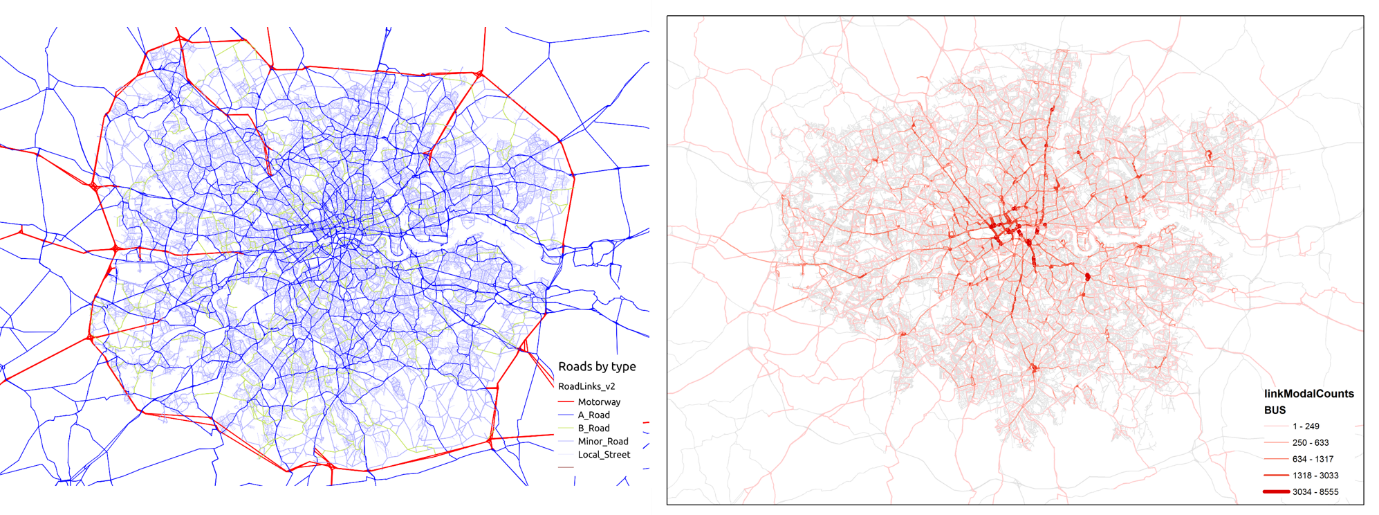
\includegraphics[width=0.95\textwidth, angle=0]{scenarios/figures/london1.png}}%
{}
% ------------
 % ------------
\createfigure%
{Visual estimate of activities performed in London at 9am using the \gls{via} software}%
{Visual estimate of activities performed in London at 9\,am using the \gls{via} software}%
{\label{fig:london_fig2}}%
{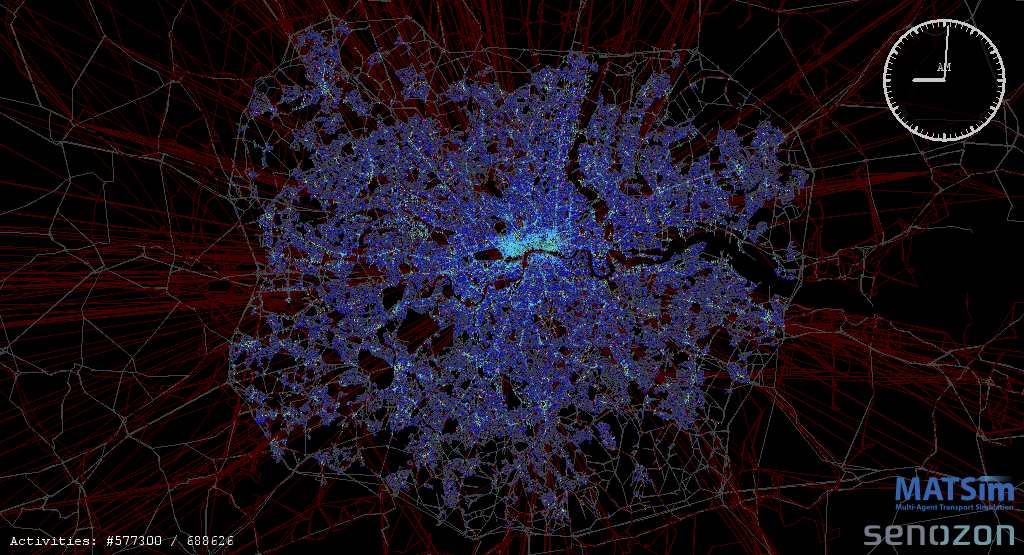
\includegraphics[width=0.95\textwidth, angle=0]{scenarios/figures/london2.png}}%
{}
% ------------

% ##################################################################################################################










